\section{3D pose estimation}
From a historical perspective, a 3d motion capture algorithm consists of 4 sequential processes: initialisation, tracking, pose estimation and recognition. Initialization involves both camera and model initialization, i.e. setting the camera calibration and finding a model that represents the subject and assigning its initial pose manually or automatically. Model-based approaches can be viewed iteratively, with each frame of the data source representing an iteration in which the initial pose is refined. Tracking is concerned with the relationship between the parts of the subject's body. This leads to segmentation of the subject from the background, representation changes, and establishing tracking in further images. The next phase, which is mainly covered in this section, is the estimation of the pose. A distinction is made between model-based and non-model-based methods, with the former requiring  \emph{a priori} a model. In that approaches, especially human pose estimation, a human model is used to benefit from its encoded information. This model can either be used indirectly, considering e.g. only general aspects such as size and structure, or it is a direct used model. Directly used models are both more detailed and offer broader benefits in regards to occlusion handling and embedded kinematic constraints. In an application, the observed object is approximated by the model, which is continuously refined with further images. Lastly, the captured motion is classified within the recognition, the last final phase of 3d motion capture. The concept of recognition is ether based in reconstruction or directly without any preprocessing. Further investigation \cite{sumi} into direct recognition revealed erroneous estimates due to the inversion of the image data, indicating that some form of preprocessing is required to eliminate false detections. Static reconstruction uses spatial data. Thus, frames are compared with previously recorded data such as templates and sillouettes to identify body postures. These are pointing, standing and sitting as well as specially defined poses. Dynamic recognition approaches, on the other hand, use temporal features. Low-level recognition, for example, relies on spatio-temporal data and motion templates. Whit that information, a walking person can be detected in the scene. High-level recognition, on the other hand, requires pose estimation data and utilises neural networks, correlation analysis and sillouet-matching. The scope of recognizable movements thus ranges from walking to carrying, putting down or removing objects, to pointing and waving, etc. \cite{summary80s}
\\
As with 2d Pose Estimation, neural networks, particularly convolutional networks, have successfully been used to achieve more accurate results than earlier methods \cite{wang_deep_2021, Chen2016, Chen_2017_CVPR, Tome_2017_CVPR, Andrikula2010, Ye2011, Martinez_2017_ICCV}. Since neural networks can be very resource intensive to compute and the architecture can be extremely complex when working with 3D data, many  of the presented approaches use 2D Pose Estimation followed by an uplifting process to 3 dimensions.  Also, a lot of 2D training data is available in comparison to 3D data which could be used to train a neural network, because the annotation process is way harder in higher dimensions. Especially the lack of in-the-wild 3D training data, which is not created under laboratory conditions, can be partly overcome by using 2D pose estimation methods (which work way better in-the-wild because of more training data available) first before adding an extra dimension.
 Therefore \cite{Chen2016} presents a process to synthesize training images and shows that neural networks training with data generated by their method are even more effective than neural networks which were trained using real images. \cite{Rogez2016} presents a similar approach.

\subsection{Lifting from 2D to 3D pose}
For uplifting, recent work has proven statistical models such as (deep) neural networks themselves \cite{Tome_2017_CVPR, Martinez_2017_ICCV}, matching the estimated 2d pose with a database \cite{Chen_2017_CVPR} or triangulation using multiple viewpoints \cite{Dong_2019_CVPR} useful. In particular \cite{Martinez_2017_ICCV} shows that even very simple deep neural networks can be extraordinarily effective for uplifting 2d to 3d pose estimations, considering both computational resources and failure rate.
\newline
Inspired by various 2d human pose estimation algorithms, many studies have employed the outputs of 2d pose estimate methods for 3d human pose estimation to improve in-the-wild generalization performance. For example, Martinez et al. \cite{Martinez_2017_ICCV} pioneered the research on lifting 2d poses to 3d space with a simple yet effective neural network. Other methods \cite{park_3d_2016, zhou_hemlets_2019, habibie_wild_2019, tekin_learning_2017} focus on fusing 2d joint heat maps from the top-down 2d pose estimation methods with 3d image cues to reduce ambiguity. The uplifting approach also makes it possible to project the calculated 3d pose to 2d again to make sure results are consistent. \cite{wang_deep_2021} In the following two important papers in this category are presented, the first one being one of the most impactful works of the last years from Martinez et al. as it showed how performant even simple neural networks can be. The second paper presented proposed a different, unsupervised method which uses generative adversarial networks and goes to show that other methods are still being experimented with having very good results too.

\begin{figure*}[!htb]
	\centering
	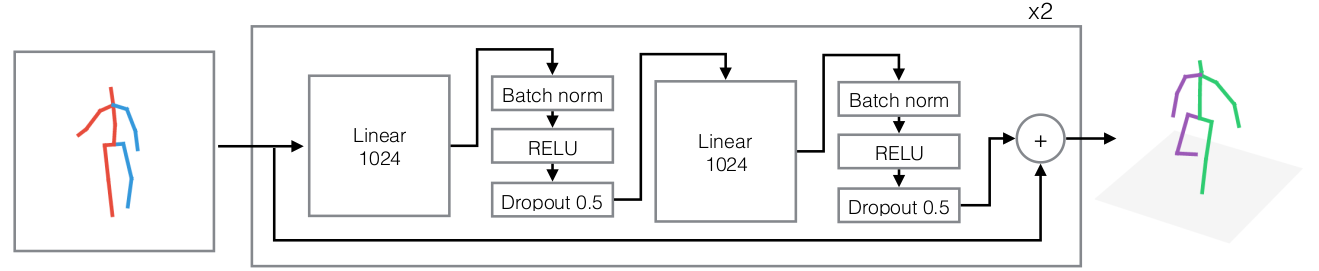
\includegraphics[scale=0.4]{3dpose/martinez_network.png}
	\caption{Neural network structure from \cite{Martinez_2017_ICCV}. It consists of two inner blocks containing a linear layer followed by batch normalization and dropout. A residual connection is added from the input of the first inner block to the output of the second. This structure is then repeated another time. The networks inputs are 2d joint positions, which it outputs uplifted to three dimensions.}
	\label{fig:martinez-network}
\end{figure*}

\begin{figure*}[!htb]
	\centering
	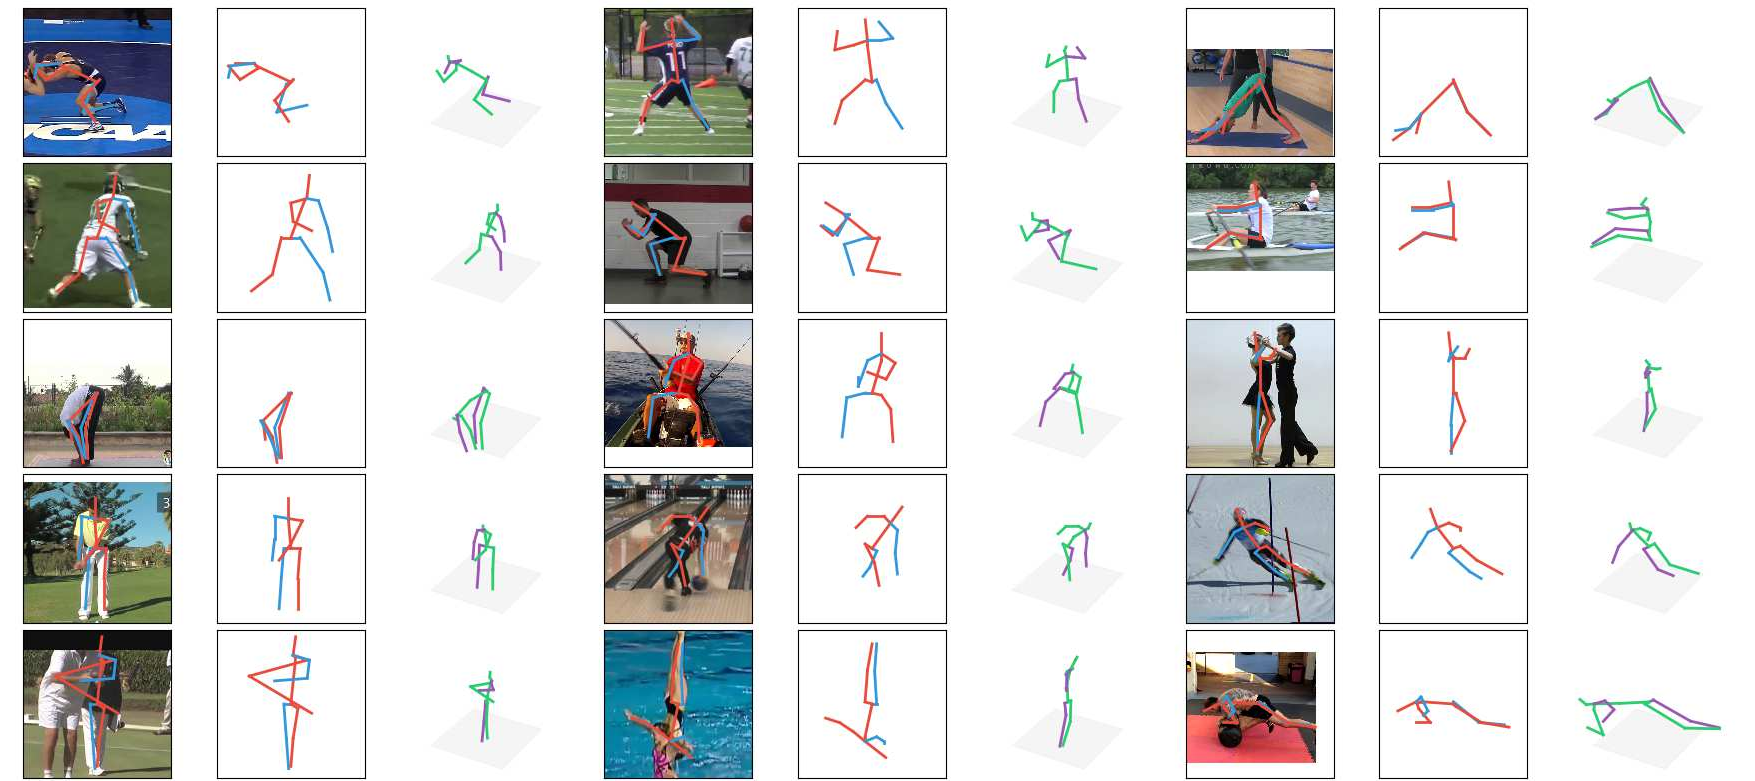
\includegraphics[scale=0.3]{3dpose/martinez_test_cases.png}
	\caption{Test cases from \cite{Martinez_2017_ICCV}. The picture on the left is the original overlayed with the 2d pose estimation (shown in the middle), while the respective uplifted 3d pose is shown on the right. Most test cases yield good results, but there are some failures too as shown in the bottom row.}
	\label{fig:martinez-test-cases}
\end{figure*}

\subsubsection{A simple yet effective baseline for 3d human pose estimation}
\label{sec:simple-yet-effective-baseline}
While trying to investigate common errors in the uplifting process, \cite{Martinez_2017_ICCV} created a method with state-of-the-art results for 3d pose estimation using a very basic neural network with recently proposed optimization methods, whose structure is shown in \autoref{fig:martinez-network}. Linear layers changing the input and output dimensions are not shown. 2d joint positions are used as input data determined by the so called stacked hourglass network as described in \cite{Newell2016}, while the output consists of 3d joint positions.\\
 Since the 2d joint positions are low-dimensional and therefore no highly complex computation is necessary, a simple linear layer with a RELU activation function is used first, followed by batch normalization and dropout as presented in \cite{srivastava2014} to prevent overfitting and improve result quality at the cost of a slight increase in computation time during training and testing. This structure is then repeated and a residual connection to the output added. These connections are proposed to help improve performance, reduce training time and lower error rates in \cite{HeZRS15}. The whole network established so far is doubled to complete the architecture which in sum consists of 4 to 5 million trainable parameters. It was then trained on Human3.6M, a dataset with 3.6 million 3d poses of humans during normal activities such as eating or walking \cite{H3.6M}.\\ Testing results show that this approach outperformed previous methods like \cite{PavlakosZDD16} in most cases, despite the simple architecture that was used. However, testing on the MPII Human Pose Dataset \cite{andriluka14cvpr} also revealed limitations of the network shown especially in the bottom row of \autoref{fig:martinez-test-cases}. Firstly (left and right picture), the 2d joint position must be detected properly. The middle picture also rendered a problem, which according to the original paper comes down to poses being not included in the Human3.6M dataset, such as upside-down poses or examples not showing a full human body.\\
 The authors conclude that basic neural networks today are already able to produce very good results in terms of accuracy for uplifting 2d to 3d human poses. Therefore one of the main error sources of this process remains 2d pose estimation and more complex models should be able to perform the task of uplifting even better.
 
\begin{figure*}[!htb]
 	\centering
 	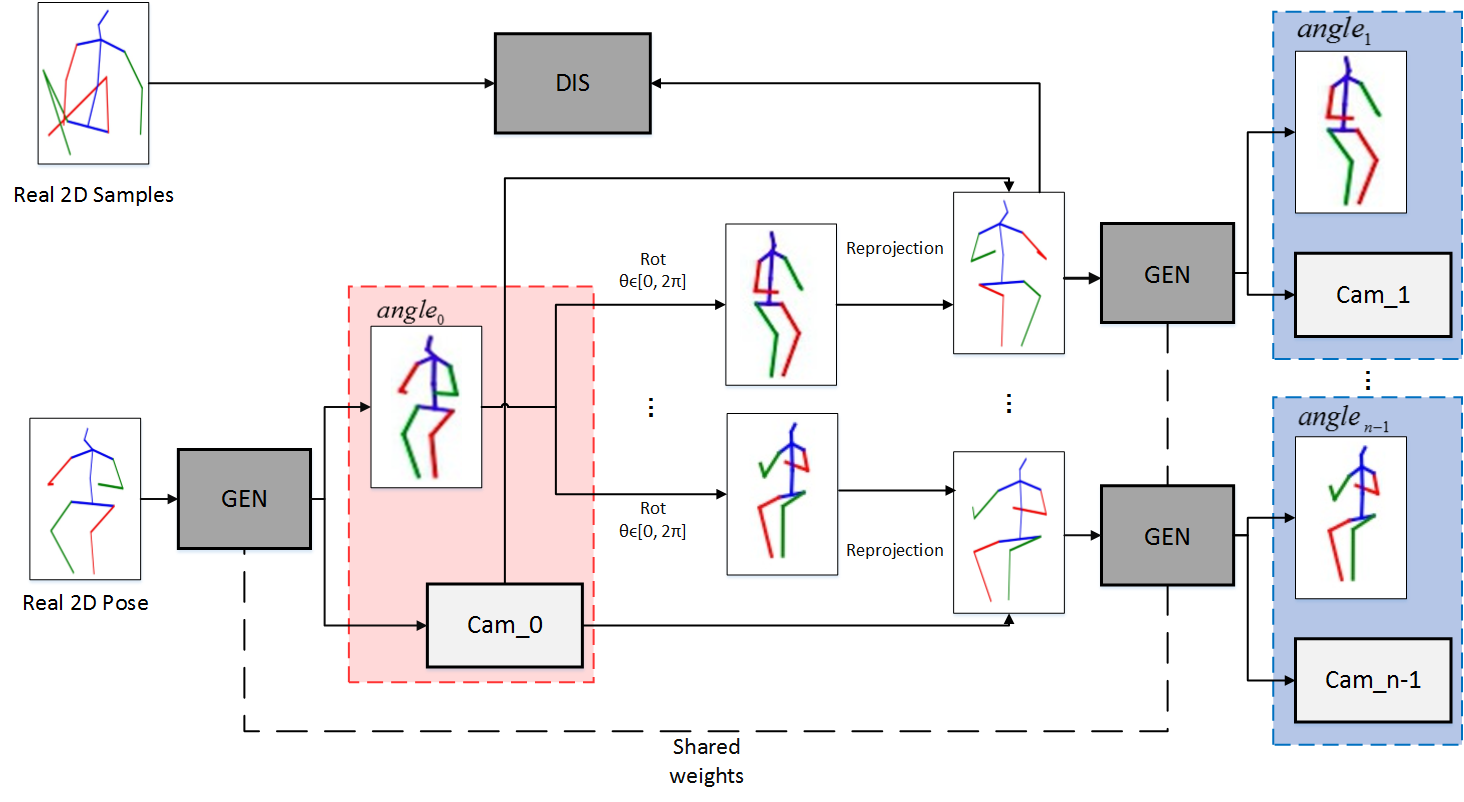
\includegraphics[scale=0.35]{3dpose/deng_main_structure.png}
 	\caption{GAN structure from \cite{Deng2021}. The input 2d pose gets uplifted to a 3d pose estimation and an estimated camera position by the generator. This allows rotation of the model to feed the discriminator with a reprojection from various angles, who is comparing them with real 2d poses. The reprojections are also used to uplift and reproject them again to ensure Single-view-multi-angle Consistency.}
 	\label{fig:deng-structure}
\end{figure*}
 
\subsubsection{SVMAC: Unsupervised 3D Human Pose Estimation from a Single Image with Single-view-multi-angle Consistency}
\cite{Deng2021} proposes a generative adversarial network (GAN) method which works unsupervised with just 2d joint positions as inputs. The generator gets trained to lift the input to a 3d pose estimation and extract the camera position, which enables rotating the model to reproject it into two dimensions. The reprojected 2d joint positions aswell as the ground truth ones are used to train the corresponding discriminator of the GAN. Single-view-multi-angle Consistency (SVMAC) denotes the ability to mix different rotations of an estimate pose with those of the estimated camera and ensuring that reprojections into 2d from the same angle are consistent. This is used in the loss function of the generator.
The structure of the network is shown in \autoref{fig:deng-structure}. SVMAC constraints are applied using the generators on the right.
SVMAC resulted in heavily improved performance of the model when using just 2 angles. However using more than 2 did not yield a significantly better result but increased training time by a lot.
Another experiment done was including 5\% ground truth data (3d poses) for supervision (with 2 angles used for SVMAC), which led to impressive results being able to outperform many weakly- and even some fully supervised approaches in terms of PMPJPE (see \autoref{criteria:mpjpe}). When considering only unsupervised methods, this one outperformed any previous one.
 
\subsection{3d pose directly from 2d image}
Methods for 3d human pose estimation directly from an imagine (or many) show the lack of 3d training data not captured by special indoor motion capture systems. This often leads to worse performance when comparing to uplifting methods in a real scenario test. If more in-the-wild datasets are coming up in the future, generating a 3d pose directly from a 2d image could be outperforming the uplifting approach. For now, generating artificial or weakly annotated training data or using multitask networks that can estimate 2d and 3d poses yields the best results in this area \cite{wang_deep_2021}.

\subsubsection{Structured Prediction of 3D Human Pose with Deep Neural Networks}
Tekin et al. \cite{Tekin2016} showed that using a separately trained autoencoder to apply knowledge about human poses and combining it with a deep neural network can improve prediction accuracy. First, the autoencoder was trained to extract poses which were prepared with gaussian noise. This resulted in the autoencoder learning constraints about human poses. The high dimensional middle layer was assumed to contain most of that information, leading to the actual CNN being trained to output this layer for the corresponding input picture. Once this training was completed, Tekin et al. added the decoding layers (from middle layer to 3d model) of the autoencoder to the network, such that the output now was an actual human pose. After some fine-tuning of the now complete CNN experiments could be conducted.
They showed that this approach led to an improvement when compared to previous methods, however their results can not keep up with uplifting methods such as presented in \autoref{sec:simple-yet-effective-baseline}. The authors conclude that the framework used is generic and therefore can be used in future projects and applied to other prediction problems.

\subsubsection{2D/3D Pose Estimation and Action Recognition using Multitask Deep Learning}
In \cite{Luvizon2018} a convolutional deep neural network structure is proposed, which is able to handle 2d and 3d pose estimation from still images plus action recognition from video, since those problems are coupled. While not achieving groundbreakingly new state-of-the-art performance results in any of the solved tasks individually, this approach goes to show that a single architecture is able to produce at least equally as good results as dedicated methods for each task separately. Since the solved problems overlap, the network can work very efficient computationally. The authors claim that merging the tasks and training them together also increases robustness. Datasets used include Human3.6M \cite{H3.6M} and MPII Human Poses \cite{andriluka14cvpr}, which render comparison with the approach presented in \autoref{sec:simple-yet-effective-baseline} possible. The multitask convolutional neural network outperforms \cite{Martinez_2017_ICCV} quite a lot, what in turn proves that complex network structures can produce even better results, as Martinez et al. stated.

\subsection{model-based 3d pose from 2d image}
The approaches to model-based estimation of human posture are either optimization-based, where a model is iteratively refined from its initial state to fit the observed object, or regression-based, where deep neural networks extract features of the image to construct the model from shape and pose parameters. The former methods allow an exact match of image and model, but are not particularly fast and sensitive to the initialization. The latter provide acceptable but not entirely accurate results, are faster but depend on their supervision \cite{spin}. \\
A common example of an optimization-based approach is found in the publication by Bogo et al. \cite{simplify} from 2016. It is the first application of \emph{SMPL} in the field of human pose estimation. The \emph{SMPLify} algorithm is based on optimization and gradually tries to align the mean initial \emph{SMPL} human model to 2d keypoints of the initial image. \\
However, \emph{HMR} is a pose estimation network, which is a regression-based method published by Kanazawa et al. \cite{hmr}. In their work, an encoder-regressor-discriminator architecture is discribed in which the encoder detects features that are regressed on pose, shape and camera parameters using an iterative regression module and finally passed on to the discriminator. The discriminator is learned from real data and has the purpose of detecting whether the parameters refer to real body meshes, so it acts as a supervisor. \\
A recent pose estimation approach is presented by Rong et al. \cite{frankmocap} which starts from the concept of splitting the estimation of human pose into hand, face and total body, which are then merged into a final model. Each aspect utilises its own regressors, which are trained on datasets selected for the respective purpose. In accordance with this separation of concerns, the different network architectures and approaches are explained in the further sections.

\subsubsection{hand estimation}
\begin{figure}[h]
	\centering
	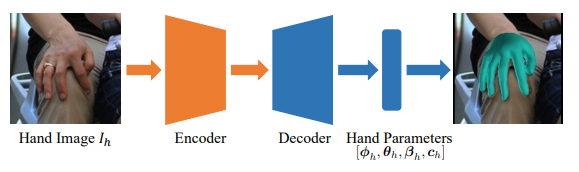
\includegraphics[width=\linewidth]{3dpose/frankmocap_hand.png}
	\caption{Encoder-decoder architecture that takes a hand image as input, extracts the features and decodes them as sufficient parameters to construct a hand model.\cite{frankmocap}}
	\label{fig:frankmocap_hand}
\end{figure}

In \emph{FrankMocap} by Rong et al. \cite{frankmocap} the estimation of human hand posture is based on regression and uses a similar structure to the \emph{HMR} shown in \autoref{fig:frankmocap_hand} with an ecoder-decoder structure. Since \emph{SMPL} does not support detailed hand shapes and postures, FrankMocap uses \emph{SMPL-X} to include this information, which extends SMPL from \autoref{sec:SMPL} to include hand movements and facial expressions. Thus, the parameters $[\phi_{h},\theta_{h},\beta_{h},c_{h}]$, i.e. the global orientation, pose and shape data of the hands, as well as the camera parameters were calculated. For the network, the annotations in the trained dataset are axis-angle representations to indicate 3D positions and 3d or 2d vertices as common positions, and therefore each annotation has its unique loss function. To increase the robustness of the model, data augmentation techniques such as random scaling, rotation, etc. and a blur filter are applied to the dataset to be learned.

\begin{figure}[!h]
	\centering
	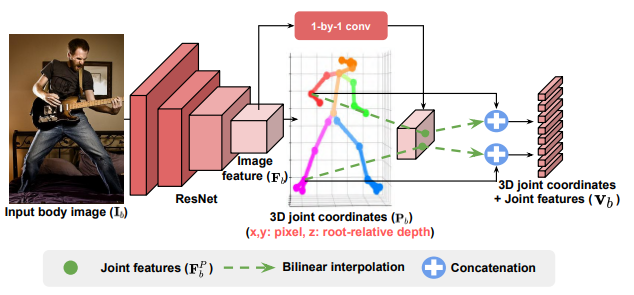
\includegraphics[width=\linewidth]{3dpose/p2p.png}
	\caption{Documentation of the \emph{Pose2Pose} structure applied to the body (b). First $\protect ResNet$ calculates the features of an input, which were used to calculate the joint positions and features with 1-by-1 convolutional layers. The features and positions were merged as input to the final layer of $\protect ResNet$.\cite{moon}}
	\label{fig:p2p}
\end{figure}

Choutas et al. \cite{expose} contributed with their approach \emph{ExPose} to overcome the limitations imposed by the small pixel area covered by a person's hands and face. In neural networks the resolution becomes even smaller, resulting in fewer relevant pixels in these areas and thus less meaningful data.
Therefore, \emph{body-driven attention} is introduced as a procedure in which the low-resolution body joints are first calculated from the pose parameters $\theta_{b}$ in order to recognise the hand and face areas in the high-resolution image. Thus, a bounding box is calculated from the corresponding hand and face joints in the low-resolution image and projected onto the high-resolution image. Finally, the high-resolution hand and face images were fed into the respective neural networks, to  refine the specific initial low-resolution pose parameters $\theta_{b}^{wrist}, \theta_{b}^{fingers}, \theta_{b}^{face}, \psi_{b}$ by adding predicted offsets. Thus, the wrist, hand and face posture as well as the expression coefficients can be represented by \autoref{eq:expose_face_hand}.

\begin{equation}
\label{eq:expose_face_hand}
\begin{split}
[\theta^{wrist}, \theta^{finger}] &= [\theta^{wrist}_{b}, \theta^{finger}_{b}] + [\Delta\theta_{wrist},\Delta\theta_{finger}] \\
[\psi, \theta^{face}] &= [\psi_{b}, \theta^{face}_{b}] + [\Delta\psi,\Delta\theta_{face}]
\end{split}
\end{equation}

Another paper by Moon et al. \cite{moon} states that the estimation of the hand depends on the prediction of the rotation of the wrist and fingers and the accuracy of the results relies on two crucial aspects. Firstly, considering the human kinematic chain, the wrist is connected to the metacarpophalangeal \emph{MCP} joints, the finger roots. Knowledge of the \emph{MCP} joints therefore benefits the calculation of the wrist and thus the estimation of the hand. In addition, the body pose can be used to determine whether the wrist rotation is anatomically correct. Lastly, the finger rotations were a product of body and hand features, which contained unnecessary information about the body and background, as well as rough information about the hand due to its small size. \\
To this end, \emph{Pose2Pose} is described as a 3d joint position guided framework for predicting 3d joint rotations. It extracts the $J$ 3d joint positions $P$ from an input image through the neural network \emph{ResNet} that encodes x and y in pixel space, while z is relative to the root joint, the wrist. The result is a feature map $F$ from which headmaps $H$ are obtained by applying a 1-by-1 convolutional layer, reducing the channel dimension of $F$ to $8 \cdot J$. Finally, the common locations are obtained by reshaping $H$ and calculating the \emph{soft-argmax} operation \cite{softmax}.\\
In order to calculate the pose parameters, joint feature information is gained by performing positional pose-guided pooling \emph{PPP}. For this purpose, a specific 1-by-1 convolution is applied to reduce the image dimensions, followed by a bilinear interpolation between the layer output and $P$, without considering the z-axis. The outcome of this practice are the joint features that, concatenated with $P$ and inserted into the final fully-connected layer of \emph{ResNet}, yield the desired pose parameters. \autoref{fig:p2p} shows the \emph{Pose2Pose} system applied to the body, which is also used for the hands in the approach by Moon et al.

\subsubsection{full-body pose estimation}
\begin{figure}[h]
	\centering
	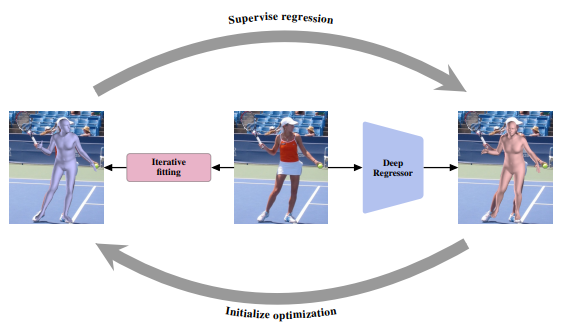
\includegraphics[width=\linewidth]{3dpose/spin.png}
	\caption{Visualisation of the $\protect SPIN$ loop, in which first the pose and shape parameters on the right side were regressed to initialize the $\protect SMPLify$ algorithm on the left side. The optimized parameters from $\protect SMPLify$ were used to improve the supervision of the regressor modul, resulting into better initial models for $\protect SMPLify$. \cite{spin}}
	\label{fig:spin}
\end{figure}

Similar to hand estimation, shape $\beta_{reg}$, pose $\theta_{reg}$ and camera parameters $Pi_{reg}$ can also be regressed in whole body pose estimation approaches. The supervision is communly processed by projecting keypoint information between dimensionens using the optained camera parameters, to use them in loss functions. An example of such a 2d loss function is given in \cite{chen} by Dongyue et al. where the ground truth joint positions are directly regressed from the neural network \emph{AlphaPose}, which are then compared to the associated joint positions resulting from the 3d-to-2d projections of the pose parameters. On the other hand, the regressed 3 dimensional information about pose and shape from \emph{HMR} are used as ground truth in 3d loss functions. As in the work of Dongyue et al, pose estimation is done by initializing the pose and shape parameters using \emph{HMR} regression and minimize the 2d loss function from which new camera parameters are calculated to finally minimize a total loss function which is the sum of the 2d, 3d and face losses. The results of this process are the pose and shape parameters. \\
The algorithm \emph{SPIN} \cite{spin} used in \emph{FrankMocap} goes further by combining the advantages of optimization and regression-based implementations by using \emph{SMPLify} and neural networks in loops. Substituting $\beta_{reg}$ and $\theta_{reg}$ into \autoref{eq:smpl} yields a human output mesh $M(\theta_{reg},\beta_{reg})$. Instead of projecting the 3d joint positions into 2d space through a pre-trained regressor based on the camera information $\Pi_{reg}$, which is then used in the loss function for supervision, \emph{SPIN} bypasses this process by calculating optimised poses $\theta_{opt}$ and shape $\beta_{opt}$ parameters through \emph{SMPLify} and uses them as pseudo ground truth in a 3d loss function. This self-impruving nature of \emph{SPIN} can be observet in a small example. \\
In the first iteration, the parameters $[\theta_{reg},\beta_{reg}]$ are regressed by a neural network, which is used to initialise the stepwise optimisation process \emph{SMPLify}. After its last step, both the pose and shape parameters are refined $[\theta_{opt},\beta_{opt}]$, resulting in an optimized body model $M(\theta_{reg},\beta_{reg})$, which is then used as ground truth in the loss function to optimize supervision of the regression module. In further iterations, \emph{SMPLify} is instantiated with a better initial model from the regressed parameters, resulting in faster and more accurate computation. The loop is also showed in \autoref{fig:spin}.\\
However, all networks, including those for the body shape and pose parameters in the work of Choutas et al. \cite{expose}, the process of \emph{HMR} is followed. \\
Finally, Moon et al. \cite{moon} intend to include the \emph{MCP} joint information as it is beneficial for body estimation. Thus, in its overall human pose estimation structure called \emph{Hand4Whole}, the hand poses were detected prior to the body. The \emph{MCP} joint features and positions can be additionally included in the posture estimation algorithm by passing them as additional values to the last phase of \emph{pose2pose}, which are then inserted into \emph{ResNet} network. \\

\subsubsection{face estimation}
As with human bodies and hands, faces also require parameters for \emph{linear blend skinning} approaches that can be regressed from neural networks. The \emph{FLAME} model, for instance, relies on shape $\beta_{f}$ and pose $\theta_{f}$ parameters as well as expression parameters  $\psi$. Thus \autoref{eq:smpl} of the \emph{SMPL} model and $T_{F}$ in \autoref{eq:Tf} can be reformulated, which is viewed in \autoref{eq:flame}. As with \emph{SMPL}, pose, shape and additionally expression blend shapes [P,S,E] must be learned. \cite{flame}

\begin{equation}
\label{eq:flame}
\begin{split}
M(\vec{\beta}_{f},\vec{\theta}_{f}, \vec{\psi}) &= W(T_{F}(\vec{\beta}_{f},\vec{\theta}_{f}, \vec{\psi}),J(\vec{\beta}_{f}),\vec{\theta}_{f},\mathcal{W}) \\
T_{F}(\vec{\beta}_{f},\vec{\theta}_{f}, \vec{\psi}) &= T + B_{S}(\vec{\beta}) + B_{P}(\vec{\theta}_{f}) + B_{E} (\vec{\psi})
\end{split}
\end{equation}

\begin{figure}[h]
	\centering
	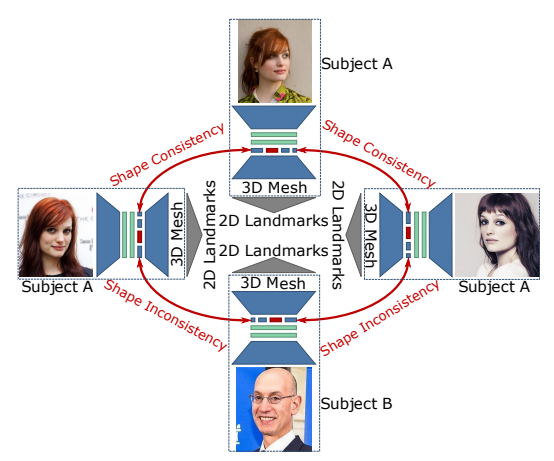
\includegraphics[width=\linewidth]{3dpose/ringnet.png}
	\caption{Ring-shaped network architecture of the $\protect RingNet$ in training with 4 elements that are encoder-decoder structures. Training is performed with image sources consisting of 2 subjects, with only one image coming from the second subject. Ring instances regress 3d information from 2d images, which are projected into 2d space for evaluation in the loss function. This concept ensures the learning of consistency.\cite{ringnet}}
	\label{fig:ringnet}
\end{figure}

\emph{RingNet} \cite{ringnet} is a regresson based approach to get the necessery parameters for the \emph{FLAME} model. It introduces a ring-shaped architecture to increase the consistency of a person's face shape across different images. During the training, the 3d landmarks of a face were calculated and projected into 2d space to compare them in the loss function with the real landmarks of the dataset, which is displayed in \autoref{fig:ringnet}. To learn consistency, a dataset provides many images of the same subject, which are then learned in a ring structure with an image of another person. Each element of the ring consists of an encoder-decoder structure, with encoders sharing weights with other encoders. An encoder calculates high-dimensional features that are iteratively regressed by the encoder's regression network in an error feedback loop. Distinctness, which consists of producing the same shapes for the same individual but different shapes for different people, is achieved by including a threshold $\eta$ in the loss function, which implies that the distance between equal subjects is always $\eta$ smaller than the distance between unequal individuals. \\



% MAYBE describe softargmax + heatmaps block for pose esti
% TODO some unsupervised or training data generation



\subsection{Direct 3d pose estimation}
Methods working directly on 3D data, such as \cite{Ye2011} (working with depth maps) can avoid potential sources of error such as projections or lighting conditions. This leads to more robust and accurate results, however more complex (neural network) architectures and computational resources are required. Traditional methods like the least-squares-estimation presented in \cite{Haralick98} work without training data needed and are computationally inexpensive, but yield rather high error rates compared to newer methods.\\